\chapter{Introduction} \label{sec:intro}

In computer graphics, most images are typically stored as a sequence of dots in a rectangular grid. Each dot is called a pixel, a small part of an image that holds one specific colour, Photographs, also called natural images\cite{hoshyari2018perceptiondriven}, are one of, if not the most, common images that are stored in this manner. Many digital forms of art or any graphics work, such as paintings, posters, and icons, are also stored the same. Digital images stored in this manner are called \textit{raster images}. These images are stored in various image formats. The most commonly used formats are JPEG, GIF, BMP, TIFF, and PNG. Each have their pros and cons, from quality of the resulting image to the file size. Nevertheless, they all still accomplish the task of holding raster image data. Everything you see in the displays of devices such as laptops and mobile devices is a raster image. Computer displays are collections of pixels, in the common definition of a dot on the screen, which computers map images to to be able display them. This is the reason why \textbf{all} \textit{displayed} images are raster images.

\begin{figure}[h]
	\centering
	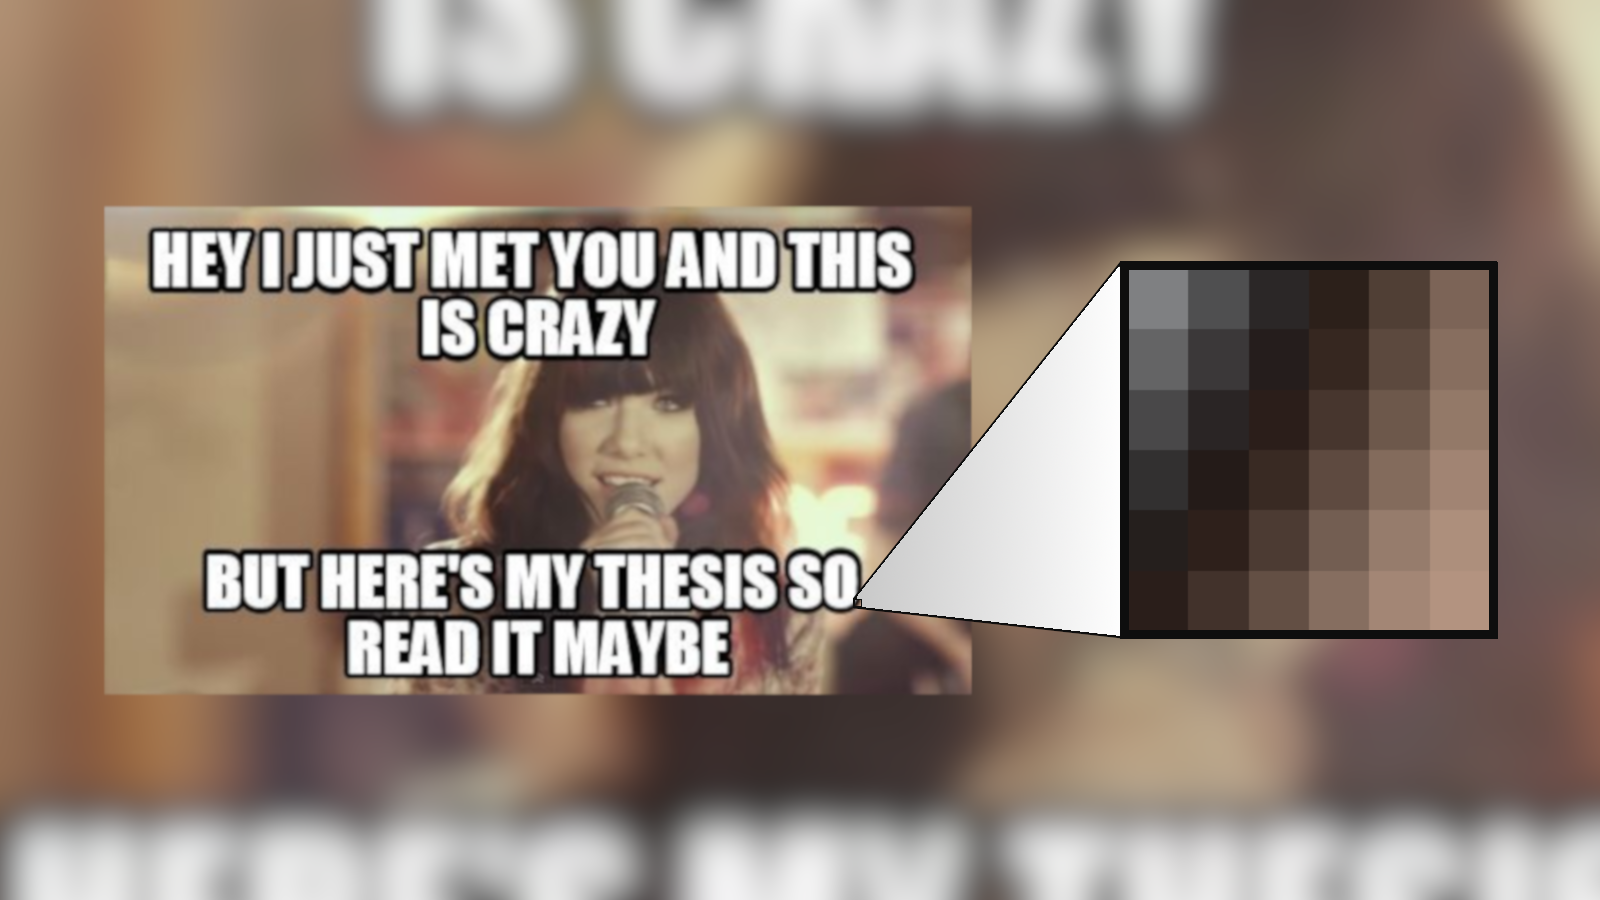
\includegraphics[scale=1.0]{images/chap01-introduction/raster-images-upclose.png}
	\caption{When zoomed in enough, each individual pixel of a raster image are visible. Original image from \protect\url{http://thesismemes.tumblr.com/post/73483120281}}.
	\label{fig:raster-images-upcose}
\end{figure}

A positive aspect of raster images is their simplicity. As mentioned earlier, raster images consists of a grid of pixels (also called a pixel matrix in other literature \cite{realtimevectorizationgpu}). This pixel grid can simply be assigned a combination of colour values to create an image. As such, working with raster images can be analogous to painting in the real world \cite{rastervsvector}. Given the right combinations of colours, we can produce natural images, i.e. photographs \cite{hoshyari2018perceptiondriven}. Intuitively, this means that we can store fine details in a raster image \cite{optimizedgradientmeshes}. This is in contrast to \textit{vector images}, which use a series of points and mathematical calculations to form lines and shapes. Vector images are unable to display lush colour depth and keep granularity, as found in raster images, as they use solid colours or gradients  \cite{rastervsvector}\cite{rastervsvectorgraphics}. There are studies that have been conducted in improving and utilizing \textit{gradient meshes}, a vector graphics primitive that allows for intricate colour gradients in regular quadrilateral meshes first introduced by Adobe Illustrator, to produce photorealistic vector images. However, as noted in the paper by Jian, S, Liang, L., Wen, F., and Shum, H., simple gradient meshes are insufficient to keep the fine details of images \cite{barendrecht2018locally}\cite{optimizedgradientmeshes}. It is also important to mention that vector graphics, despite represented as mathematical calculations, are still converted to raster format in a process called \textit{rasterization} for it to be displayed on-screen, since many modern screens are raster displays \cite{howdovectorgraphciswork}.

\section{The Problems of Raster Graphics}


% Talk about AI Gigapixel but still state the problem with rasters being resolution-dependent.

% Include the reason where you say that vector images are still rasterized before being displayed.

% Note: Maybe add here why raster images are simple in the context of image processing once we learn more about image processing.